\documentclass[a4paper,11pt]{article}
\usepackage[margin=1.2in]{geometry}
\usepackage{titlesec}
\usepackage{graphicx}
\usepackage{caption}
\usepackage{subcaption}
\usepackage{wrapfig}
\titleformat{\paragraph}
{\normalfont\normalsize\bfseries}{\theparagraph}{1em}{}
\titlespacing*{\paragraph}
{0pt}{3.25ex plus 1ex minus .2ex}{1.5ex plus .2ex}
\fontfamily{cmss}\selectfont

\author{
  Ernst, Matthew\\
  \texttt{ernst183@umn.edu}
  \and
 Isava, Manuel\\
  \texttt{isava001@umn.edu}
\and
  Saari, Nicholas\\
  \texttt{saar0096@umn.edu}
}

\title{Probabilistic AI in Bullshit Card Game}
\linespread{1.15}

\begin{document}

\maketitle



\begin{abstract}
Probabilistic artificial intelligence is a powerful tool for creating card game players. One such card game, Bullshit, is an interesting game due to the impossibility for the players to perfectly track cards and due to the ability of players to bluff cards. Therefore, this game creates a good scenario to use a probabilistic artificial intelligence agent to play the game. This kind of AI is useful because it is able to calculate the probabilities relevant to the current game state and then make decisions based on those probabilities. In this paper we implement such an agent for the Bullshit card game, with different evolution or improvement stages; more specifically, we implement an agent that calculates the probability of an adversary’s move based or given the current evidence the agent possesses and its belief state, that is, the agent’s belief of what cards the respective adversary has in its hand and what cards he believes are in the pile. We demonstrate that building an agent that is successful against different kinds of opponents is a difficult task to accomplish, given the high level of uncertainty present in the game.
\end{abstract}

\section{Introduction}
	Before dwelling in depth into the specifics and findings in this paper, it is necessary to give an overall introduction and description of the Bullshit game for the unfamiliar reader. Bullshit is a card game where the goal is to empty your hand using previous knowledge, luck and bluffs. The game plays in a cyclic order with each player being designated a card value on their turn, starting at one (ace) for the first player and going up one each turn afterwards. Each player must play one to four cards of any value. Then, the rest of the players get the chance to call “bullshit” or “BS.”  If nobody calls BS, the cards simply remain on the table and the next player takes his/her turn. If a player calls BS, the  cards played by the player whose turn it is are revealed. If all of the revealed cards are equal to the value that the player was assigned for his/her turn, whoever called BS must pick up the entire pile. If there is at least one card that does not match the value, the player that played the cards must pick up the entire pile. This continues until one player is able to empty their entire hand. Whoever empties his/her hand first is the winner.

The inherently probabilistic nature of this game makes it a very appealing subject of research and it was the main motivation for the work done in this paper. The structure of the paper is divided into different sections, more specifically,  in section 2 we present and discuss previous works about probabilistic card game agents, like poker. In section 3 we present some interesting findings about the fairness in the structure of the game that has to do with the number of players and the ordering. In section 4 we discuss in depth the experimental setup and the strategy we chose for the different tests’ environment. In section 5 we provide and analyze the results obtained during the experimental and testing stages. Finally, Section 6 we present our final conclusions and interesting findings. 


\section{Literary Analysis}

A paper that we found useful towards this project was “Using Probabilistic Knowledge and Simulation to Play Poker.” This paper, published in 1999, explores using artificial intelligence to play games with hidden knowledge, such as most card games \cite{billings}. Specifically, they explore the game of poker, since it is a highly probabilistic game with a large amount of hidden knowledge. The researchers created a program named “Loki” that was a reasonably strong poker player. They built Loki using a number of modules, the Bettor, the Hand Evaluator, and the Opponent Modeler. The Bettor used “expert-defined rules and hand assessment provided by the Hand Evaluator for each betting decision: fold, call/check or raise/bet” \cite{billings}.  The Hand Evaluator evaluates Loki’s hand and uses it to determine how good of a hand it has and what kind of hands it should expect opponents to have. The Opponent Modeler uses information from the Hand Evaluator to determine the probabilistic strengths of the opponent’s hands. While this was not their final product, this set-up much more closely resembles how we wanted our AI to approach the problem, since there was no real “betting” statistic in BS.

	The paper continues to talk about how they iterated through a few different versions of Loki, each slightly changing Loki’s setup, using different systems to simulate games and increase their win percentage. The paper focuses on three enhancements to Loki, the changing of the re-weighting system to use probability triples, changing from a rule-based bettor to one that uses probability triples, and uses a simulator to compute an expected value estimate for a bet \cite{billings}. Each of these enhancements had varying effects on the agent’s success. The first two changes each had about the same effect on its win rate against the basic Loki player. Having both of them together gave approximately double that advantage. The third change alone gave almost double the advantage that the first two changes gave together. Adding the first to changes to the third change gives a very small advantage over only the third change. 

	This paper, while strong in the sense of exploring different options, runs into an issue of data representation. A difficult thing to do when building a game AI is to show that is is actually a strong player of the game, instead of just a strong player against a specific opponent. They do not seem to take into account that their testing was done purely against the first iteration of Loki, leading to much of their actual data sampling to be questionable, as their measurements of success might just mean it’s good at playing against Loki-1 more than meaning that it’s good at being poker. However, they counteract this issue well by teaching Loki to play on an online poker server. On the poker server, against human players, Loki gets to show that it is actually a strong player or poker, as it is able to beat all manner of players fairly consistently. This use of human testing shows a much better comparison of strength for Loki, as inconsistent human players (both good and bad) are able to test its skill much more than playing against Loki-1 twenty-five thousand times.

	Overall, this paper is a good exploration of AI used in games with hidden knowledge and sets up a good strategy for approaching problems of this nature. It succeeds in creating a fairly strong poker player and finds different ways to change this agent to increase its strength even further. They manage to overcome the issue of testing the strength of their player by testing it against a large number of human players of variable strength. This paper was useful in setting up our own AI for BS and gives us some things to look into to improve our own AI in the future.

It is clear that modeling uncertainty is difficult\cite{koller}. Others have used Monte Carlo Search to model card games relatively successfully \cite{van}. Many of our design choices do not follow in the footsteps of other projects, but are very specific to the game of Bullshit. Furthermore, while many individuals have modeled poker \cite{van} \cite{billings} , where there are a plethora of online gaming statistics and previously developed strategy, we trudge ahead blindly. The amount of unavailable information makes the use of either a tree \cite{slantchev} or a Bayes network \cite{milch} unattractive due to the branching factor and complexity respectively.

\section{Interesting Findings in Fairness and Ordering}
	Our first experiments with the game Bullshit consisted of running players that would play the correct cards if possible and bluffing with one to four random cards from their hand otherwise; such agents would also call BS 50\% of the time. We found that as long as the player list is shuffled after each game (meaning that the order of players is random each game), the game is even. However, if you do not shuffle the game and there are an even number of players, some players will completely dominate the game. For example, in a four player game, players one and three show a significant advantage over player two and four, often each taking about one third of the wins each, with players two and four getting about one sixth each. In Figure 1, you can see a 1000 four-player game sample of an unshuffled player list. Figure 2 shows the sample of a 1000 four-player games with a shuffled player list after each game, leading to even win-rates between players.



\begin{figure}[h]
  \makebox[\textwidth]{%
    \begin{subfigure}[t]{0.59\textwidth}
      \centering
      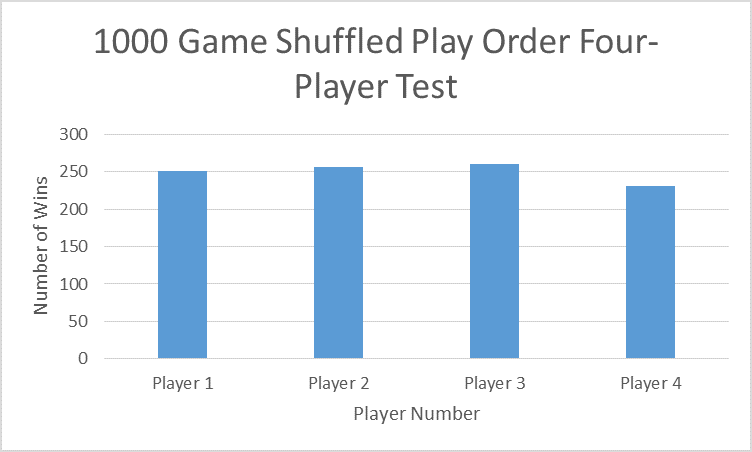
\includegraphics[width=\textwidth,height=.65\textwidth]{Shuffled_Play_Order_Tests}
      \caption{Shuffled Control Players Results}
    \end{subfigure}%
    \hfill
    \begin{subfigure}[t]{0.59\textwidth}
      \centering
      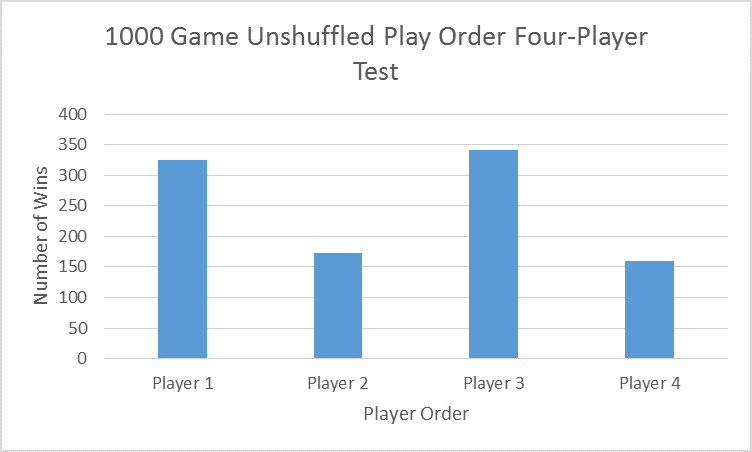
\includegraphics[width=\textwidth,height=.65\textwidth]{Unshuffled_Play_Order_Tests}
      \caption{Shuffled Control Players Results}
      \label{fig:free-lunch}
    \end{subfigure}%

  }%
\caption{Control Tests}
\end{figure}


	 This knowledge was useful for testing and building the different kind of agents we implemented, as it helped us to avoid false successes, over-modeling and leading them to only play well when playing in certain spots in the player order. Due to the advantage that certain player positions seem to give, we could be tricked into thinking that such agents were working incredibly well when really they were simply taking advantage of their spot in the player list. Thus we decided to shuffled the player list after each game for all sampling we do for the remainder of our testing to avoid this from affecting the data gathered.

\section{Experimental Setup}
	We chose to use probabilistic artificial intelligence for this problem because it fits the scenario that the game Bullshit sets up very well. Probabilistic AI is very useful in environments where there are unknowns. In the case of Bullshit, these unknowns amount to how the opposing players will act, what cards the opponents played, or whether the opponent bluffed or not. Using a probabilistic agent to calculate these probabilities and play according to what is statistically the best move should result in an optimal or ideal win rate against any non-perfect opponent. Probabilistic AI makes decisions based on measured probabilities in the environment, which allows our agent to respond to the ever changing probabilities in the game of Bullshit, by calling BS when the probability that someone has a set of cards is low and bluffing when it knows that the chance of someone calling BS on it is low. We believed that this aspect, paired with an AI’s ability to easily track played cards, should result in a very strong Bullshit playing agent. 


	\subsection{Evolution}
	Creating an agent to play Bullshit is simple. Only two functions need to be implemented: chooseCards() and callBS(). The only two actions that an agent may take when presented with a BS proposition are True (call BS) or False (do not call BS). Selecting cards to play when their turn comes is a bit more complicated. They may either tell the truth by playing the next sequential card, or bluff by playing other cards and passing them off as the proper value of card. The first step towards building our final BS agent consisted on implementing a variety of agents for testing purposes; we call this set of agents the control set or more interestingly “amphibians”.

	\subsubsection{Amphibians/Control Set}
	In order to begin our path towards creating an AI that excels at Bullshit, we needed to create simple players. This accomplished two goals simultaneously. First, training players were needed. A massive amount of trial initialization went into creating the initial pair of intelligent agents, which will be discussed as this section progresses. Second, we needed basic agents to build off of. Games between these basic (but not necessarily “bad” players) were simulated to determine which attributes were vital to winning a game. A hierarchy of agents was built from the bottom up, and the amphibians formed the bottom level of the Bullshit agent society.

	\paragraph{Fish}
	The first basic agent implemented was denominated Fish and is the worst agent of the hierarchy. Such an agent simply plays a random amount of random cards from their hand. The constructor takes a value from 0 to 1, which is the percentage of time that it will call BS when given a proposition. When the agent is asked to call BS, a sample is taken and BS is called or not based on the sample. Obviously this is not a good strategy for playing the game, and this agent will only win a few games out of 1000 due to inherent chance and randomness in the game. The caveat with this is that when pitted against fully conservative players, one that never or very rarely calls BS, the Fish will retain a very high win rate. Our first major development begins here. This approach can easily be thwarted by always calling BS whenever any player plays their final card. This is optimal play, because there can only be reward gained. Either the game ends, or the game persists because that player did not win. Due to the random playing of cards propagating through turns, chances are that every time the Fish plays its final card it is not the correct one. Against honest players who always call BS on the last turn, the Fish only experiences a win rate of approximately 10 out of 10,000 games. 

	\paragraph{Frog}
	Frog is the second most basic agent and the first one in a series of “honest players.” To be denoted as an honest player means that on the agent’s turn, if the agent has a card or cards of the proper value, it will always play all the cards with that proper value. For instance, if an agent needs to play aces, and has three aces in its hand, it will play those three aces, nothing less or more. Honest players will still need a bluff strategy for the instance when they do not have the proper valued cards in their hand. This honest trait is highly desirable, and later in the paper we explore whether it is fully optimal to be fully honest whenever possible. Frog explores a simple bluff strategy. When no card is the proper value, a single card is selected at random and played. For calling BS, the Frog is the same as the Fish. 

	\paragraph{Eel}
Eel is the third most basic agent and the second one in the series of honest players. Such an agent uses an honest strategy when it can, but is more complex when it comes to bluffing. If an Eel does not have the proper card and its hand size is less than 3, it chooses to bluff one random card with probability 1; otherwise, if its hand size is bigger than 3, it chooses to bluff one random card with 0.7 probability, two random cards with 0.2 probability and three random cards with 0.1 probability. When presented with a BS challenge, it calls BS either if the opponent tries to play more than four cards or attempts to play his last card. If none of the previous conditions hold, then the agent follows the same strategy for calling BS as the Fish and the Frog, that is, by sampling. The Eel plays well, but predictably so. Eels are easily defeated by smart players despite their relatively strong strategy.

	\paragraph{Salamander}
	Salamander is the last agent from the control set and is the last one in the series of honest players. Such an agent uses a simple strategy, but it turns out it is a very good one. Salamander plays honestly and only bluffs a single card when he cannot play honestly. Salamander only calls BS on two conditions: when the opponent plays his/her last card, and when an opponent attempts to play more than four cards. Both conditions lead to opponents with very high bluff rates to be thwarted. However, an opponent will be able to play any mix of cards on the bluff during a non-final turn and the Salamander will not catch it. 
		
\subsubsection{Smarter Agents}
	Improvements upon the amphibians in attempt to find a more optimal player lead to the development of two different styles of agent: one that focuses on bluffing and one that focuses on calling BS. The idea behind this decision was to come up with two different agents that excel at what they do, that is, one agent that is good at calling BS on adversaries and another one that is good at choosing what cards to play, and then finally combine both agents to produce a final optimal player. This lead us to implementing two new agents called “Owl” and “Lynx”; the first one focuses only on calling BS, while the second one focuses only on choosing what cards to play. Finally we combine the separate functionalities of both agents to produce a final agent called “Dolphin”.

	\paragraph{Owl}
	The Owl agent focuses only on calling BS on other players. Such an agent does so by calculating the probability of the rival’s move, that is, when an adversary makes a move, the Owl calculates the probability of that player having the cards he/she claims to have given five different kinds of information: the cards the agent belief are on the pile, the cards the agent knows are in the pile with probability 1, the number of cards that rival has on his/her hand, the cards the agent knows are in that rival’s hand with probability 1 and the cards that the agent has in its own hand. The Owl agent uses two kinds of information in order to make its decisions: the agent’s belief of people saying the truth, we call this parameter “beta”, and an upper bound in probabilities, we call this parameter “alpha”. The beta parameter is used to weight the conditional probabilities calculated based on the agent’s belief that people say the truth in order to come up with an effective probability. The alpha parameter is used as a threshold whenever the agent is presented with the opportunity to call BS, that is, if the probability the agent calculates for the move just made is below the threshold, the Owl agent calls BS, otherwise it does not. For playing cards, the Owl follows a simple strategy: it plays all the cards it has of the current card he is supposed to play if it has any, otherwise it just bluffs one random card. In this sense, we keep minimal the influence of the strategy associated with playing cards because we are only focused in the BS aspect of the game.

	\paragraph{Lynx}
	The Lynx agent focuses on bluffing, more specifically, it takes into consideration when to bluff and which cards specifically to bluff, depending on te circumstances. Such an agent uses three different pieces of information that are provided to the constructor: BS Probability, Gamma, and Gamma rate of change. When calling BS, the Lynx acts just as the Eel does with one added test, by sampling against the BS Probability. The agent adds up the total number of cards in its hand with the needed value and checks if it is indeed possible that the adversary has the number of cards he says he does. If not, BS is called. The main strength in the Lynx lies is its ability to look ahead turns and bluff intelligently. This is done by computing turns modulo 13 until a loop is formed. The cards in its hand are organized in its hand in a fashion such that the first card will be needed soonest, and the last card will be needed the furthest in the future. This way, when a bluff is played, it is played such that the cards not needed soon are discarded first. Of course, it plays honestly when it can. The twist, in this case, is that the Lynx tracks the number of times opponents call BS. The Gamma parameter changes the threshold at which the BS rate of other players must sink below in order for the Lynx to deem it safe to bluff extra cards. The Gamma rate of change parameter affects how much the agent learns by bluffing. When an agent bluffs extra cards (either on top of an honest play or on top of another bluff) it checks whether any other player calls his bluff. In the event that the bluff succeeds, the threshold is lowered by the Gamma rate of change. In the event that the bluff fails, the threshold is raised. In this way, if the game continues long enough the agent has an opportunity to learn from the way its opponents call BS against his bluffs. As expected, when the game is lengthened by adding a second deck, this agent improves against players who play one or few cards every turn. 

\paragraph{Dolphin}
This final agent consists of combining the independent functionalities of the Owl and Lynx agents. An added functionality resides in deck tracking ability. Every time the agent plays a card, it knows that that specific card is in the deck. This attribute can be helpful deciding whether or not to call BS at any given time. If the number of cards in the agent’s hand added to the number of known values in the deck added to the number of cards the opponents claims to have exceeds the total number of cards with that value, that player is obviously lying. Experiments were run with tracking known and unknown cards in the opponent’s hands, but the level of uncertainty was too great. Every time an opponent played any card from their hand after picking up known cards, the known cards in the opponent’s hands cannot be determined without knowing for certain which card the opponent played. This agent was determined to be the most effective agent created in the largest variety of situations. Win Rate gain, however, did not improve as substantially as hoped when combining the owl and Lynx agents together. 

\subsection{Experimental Environment}
For the experimental environment we decided to test the performance of the Owl and Lynx agents separately against the agents in the control set or “amphibians”. More specifically, the following set of tests were carried out for both the Lynx and Owl agents for different values for the respective agent’s parameters in a given range:
\begin{itemize}
\item 500 games with one instance of smart agent (Lynx or Owl) and 4 instances of Fish agent with BS probability between 0.05 and 0.5.
\item 500 games with one instance of smart agent (Lynx or Owl) and 4 instances of Frog agent with BS probability between 0.05 and 0.5.
\item 500 games with one instance of smart agent (Lynx or Owl) and 4 instances of Eel agent with BS probability between 0.05 and 0.5.
\item 500 games with one instance of smart agent (Lynx or Owl) and 4 instances of Salamander agent.
\item 500 games with one instance of smart agent (Lynx or Owl) and one instance of each of the players in the control set, that is, one instance of Fish agent, one instance of Frog agent, one instance of Eel agent  (all these with BS probability between 0.05 and 0.5) and one instance of Salamander agent.
\end{itemize}

\section{Experimental Data and Analysis}

\subsection{Performance of Owl Agent}
In this section we present and analyze the data gathered from the experimental environment presented in the previous section taking the Owl as our choice of smart agent. More specifically, the tests were run for different values of beta and alpha in order to find the optimal values for such parameters and analyze their influence in the agent’s win rate and rate of success when calling BS. For each of the tests, we used different values for alpha in the range [0.00, 0.2] with increments of 0.01 and we used the following values for the beta parameter: 0.2, 0.4, 0.6, 0.8 and 1.

\subsubsection{Fish as Rivals}

\begin{wrapfigure}{r}{0.6\textwidth}
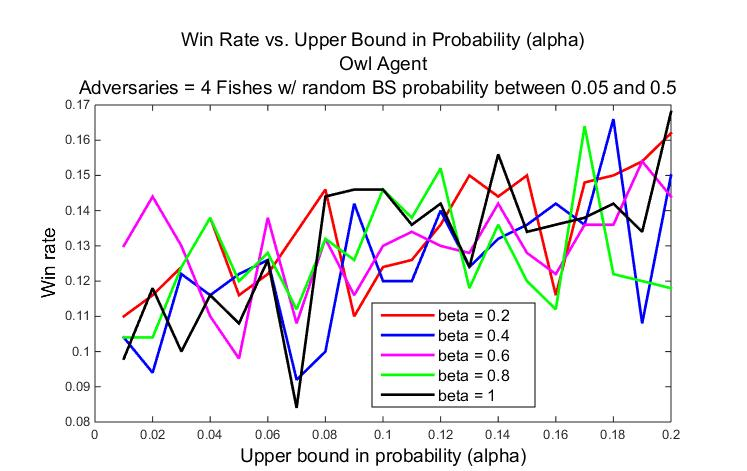
\includegraphics[width=0.6\textwidth]{owl_vs_fish_upperbBoundProb}
\caption{}
\end{wrapfigure}
	As can be seen from the graph, there is little variance in the win rate for different values of beta, approximately 0.04, this hints to the fact that the agent’s belief of people saying the truth has no relevant impact in the agent’s win rate. On the other hand, as we increase the value of alpha, the agent’s win rate increases. This can be explained by the fact that the Fish agents only make random moves, so cards are randomly being passed over from player to player, which increases the chances of a player having a given card, thus is desirable to have a higher value of alpha, that is, a higher threshold for the probabilities. Another point of interest is the low win rate of the Owl agent against this type of player; we find these results surprising and believe it is due to the fact that the random choices made by the enemy agents have a huge negative impact on the Owl’s probabilistic calculations, resulting in a cascading effect that results in probability estimates that have a huge variance with respect to the actual ones.



\subsubsection{Frogs as Rivals}

\begin{wrapfigure}{l}{0.6\textwidth}
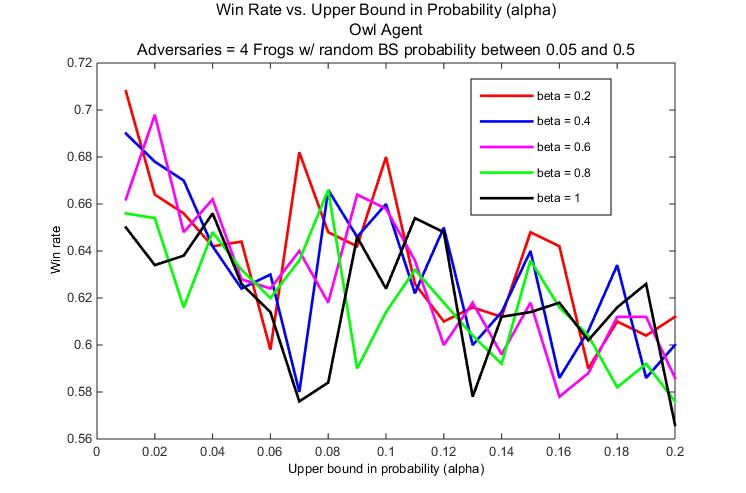
\includegraphics[width=0.6\textwidth]{owl_vs_frog_upperBoundProb}
\caption{}
\end{wrapfigure}

As can be seen from the graph, in this case too there is little variance in the win rate for different values of beta, approximately 0.06, this again hints to the fact that the agent’s belief of people saying the truth has no relevant impact in the agent’s win rate. On the other hand, as we increase the value of alpha, the agent’s win rate decreases. This can be explained by the fact that the Frog agents actually make rational decisions when playing cards, thus it is in the best interest for the Owl agent to call BS only when it is certain that the move just made by an enemy player is a fallacy. Also, it is important to notice that for optimal values of alpha (around 0.02) the win rate of the agent is good, around 70\%.

\subsubsection{Eels as Rivals}

\begin{wrapfigure}{r}{0.6\textwidth}
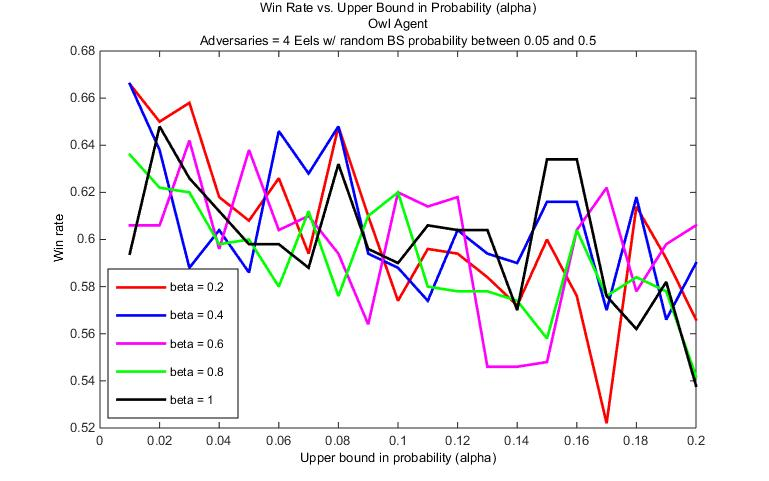
\includegraphics[width=0.6\textwidth]{owl_vs_eel_upperbBoundProb}
\caption{}
\end{wrapfigure}

As can be seen from the graph, in this case too there is little variance in the win rate for different values of beta, approximately 0.06, this again hints to the fact that the agent’s belief of people saying the truth has no relevant impact in the agent’s win rate. On the other hand, as we increase the value of alpha, the agent’s win rate decreases; this decrease in the win rate is less than when playing against Frog agents. It seems that when playing against enemies that play honestly, that bluff conservatively and that call BS with a certain probability, the value of alpha (the upper bound in the probability) has not a significant influence in the agent’s win rate.  Also, it is important to notice that for optimal values of alpha (around 0.02) the win rate of the agent is still relatively good, around 65\%.


\subsubsection{Salamanders as Rivals}

\begin{wrapfigure}{l}{0.6\textwidth}
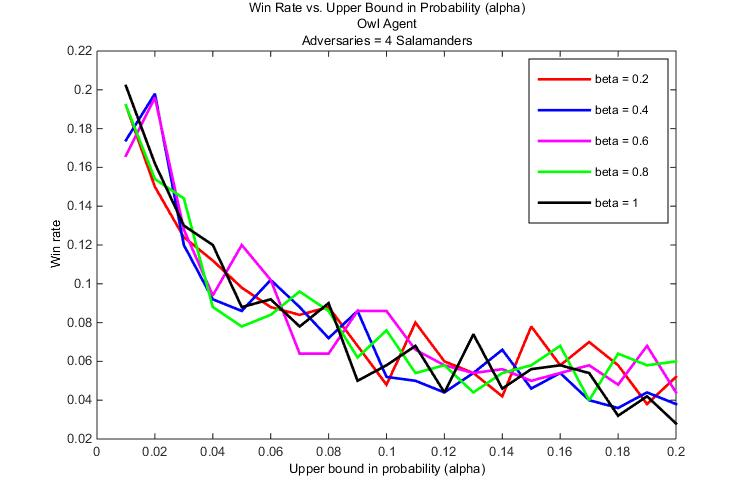
\includegraphics[width=0.6\textwidth]{owl_vs_salamander_upperbBoundProb}
\caption{}
\end{wrapfigure}

As can be seen from the graph, in this case too there is little variance, even less than before, in the win rate for different values of beta. This again hints to the fact that the agent’s belief of people saying the truth has no relevant impact in the agent’s win rate. On the other hand, as we increase the value of alpha, the agent’s win rate decreases logarithmically. So it seems that when playing against very conservative and honest players that never call BS, it is in the best interest of the Owl agent to call bullshit only when it is absolutely certain that the enemy is lying; this explains why the agent has a better win rate for small values of alpha. Another point of interest is the low win rate, below 20\%,  of the Owl agent when playing against this type of adversary. This can be due to the fact that since the enemies never call BS, they do not risk picking up the pile, while the Owl agent, even though it might call BS with small probability, still risks picking up the pile, which can cost it the game. 

\subsubsection{Variety of Rivals}

\begin{wrapfigure}{r}{0.6\textwidth}
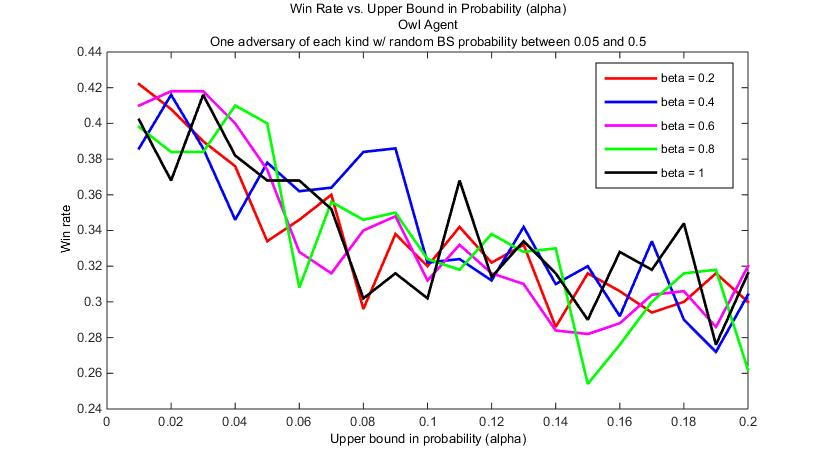
\includegraphics[width=0.6\textwidth]{owl_vs_all_winRate}
\caption{}
\end{wrapfigure}

As can be seen from the graph, in this case too there is little variance in the win rate for different values of beta;  this again hints to the fact that the agent’s belief of people saying the truth has no relevant impact in the agent’s win rate. On the other hand, as we increase the value of alpha, the agent’s win rate decreases almost linearly. This finding reinforces the belief that in this game it is best to call BS only when we are absolutely sure the enemy is lying. Also, it is important to notice that when playing against a mix set of adversaries the Owl agent does relatively good for optimal values of alpha, it wins approximately 40\% of the games. 

\subsubsection{Influence of BS Success Rate and Alpha in Agent's Win Rate}
From the previous experiments it seems to be the case that an agent’s belief of people saying the truth does not affect the win rate of such agent. This can be seen in Figure 8, which shows the BS success rate of the Owl agent for different values of beta against different types of opponents. One might think that the belief or probability of people saying the truth affects an agent’s  success rate of BS challenges, that is, the number of times the agent wins a BS challenge out of the total number of BS challenges such agent made, but our data suggests the opposite, that is, that such belief does not have an impact in the accuracy of won BS challenges. Another interesting finding that can be observed when taking Figure 7 together with the previous Figures is that an agent’s win rate is not necessarily dependent of its success rate in BS challenges. For example, the success rate of BS challenges for the Owl agent when playing against Fish adversaries is 100\%, but its win rate is low (less than 20\%). One would expect that if the agent is winning every single BS challenge, then it would win the game, but this seems to not be necessarily true.

\subsection{Performance of Lynx Agent}
This section presents and analyzes the data gathered using Lynx as the agent. Experiments were run in order to optimize values of gamma and gamma rate of change such that the Lynx is most versatile against all types of challenger.
In order to optimize these values, chinks of 500 simulations were run against varying opponent types. Gamma was varied in the range [0.9, 0.99] in increments of 0.1, while gamma rate of change was varied from [0, 0.05] in increments 
of 0.01. Earlier experiments showed that a BS Probability of 0 is optimal against amphibian test agents, due to the random nature of their play. However, BS rates of 0.08 and 0.16 were explored in these experiments, since a real agent 
needs to be able to defend against a player who simply bluffs many cards every turn. 


\subsubsection{Fish as Rivals}

Experiments with the Fish revealed almost nothing about gamma and gamma rate of change. The Lynx makes swift work of fishes as expected, winning around 95\% of games. For all values of gamma and gamma rate of change, a negligible
difference can be seen in outcome. Change in win rate is attributed to natural variance. It is clear that when purely random moves are made by opponents, it matters not how many cards are bluffed, honesty is more important.

\subsubsection{Frogs as Rivals}

Frogs, again did not provide accurate information about optimizing either parameter of the Lynx agent. Lynx plays well against the frog for a range of values, and there is clearly no trend for either parameter. Lynx wins many extra
BS challenges due to the counting of its own cards against their opponents claimed cards, and bluffs well at a variety of bluff thresholds and learning rates. 

\subsubsection{Eels as Rivals}

\begin{wrapfigure}{l}{0.6\textwidth}
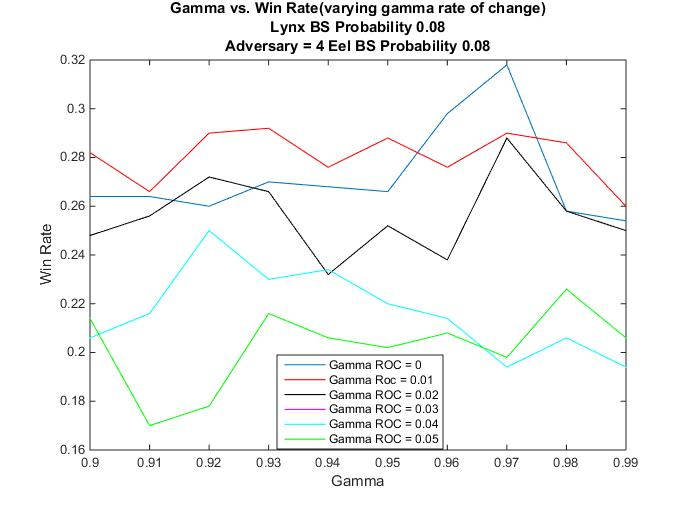
\includegraphics[width=0.6\textwidth]{lynx_vs_eel_2_gamma}
\caption{}
\end{wrapfigure}

Experiments with the eel were the most revealing set of experiments run. It is noted that the BS Probabilities of the Eels were set to 0.08, and this differs from all other experiments. The reason for this is was that the Lynx plays most similarly to the Eel out of all the amphibian agents. Setting their BS Probabilities to identical values reveals exactly how much advantage can be gained by using the learning parameter to bluff and playing with future turns in mind. As shown in fig. 7, when playing against the Eels, a gamma rate of change closer to 0 desirable. As gamma rate of change is increased, win rate decreases. Gamma represents
a learning rate, and when the lynx agent learns more slowly over time, over-analyzing is less likely. If many bluffs are made early in the game, such as typically happens with the Eels using random BS probabilities, the Lynx increases gamma well over 1, meaning no bluff cards are ever added. As gamma rate of change nears .05, the Lynx behaves almost identically to the Eel. A win rate of 0.4 is quite high against semi-intelligent agents in Bullshit, which depends on chance so much.


\subsubsection{Salamanders as Rivals}

Performance of Lynx against salamander is poor. Salamander turns out to be the most difficult player to beat as an AI. Lynx experiences a below average win rate for Salamander opponents ($\approx0.15$). The only way to combat a full group of adversaries that never calls BS is to not call BS. A Lynx can be tuned to beat Salamanders,
but in doing so performance against all other types of adversary decreases dramatically. It is clear from the graph that gamma and gamma rate of change is ineffective in the normal "good" range of values. Changing gamma to a very low number, or subsequently raising the learning rate allows Lynx to have a better chance at victory. While the results are disheartening, we continued onward with experiments assuming that this situation is rare. If all players do not call BS, the game becomes uninteresting.

\subsubsection{Variety of Rivals}


Performance against a variety of one of each type of adversary is good. A slight correlation was found between higher values of gamma and lower learning rate. That is, when other players are calling BS Fairly often, it makes sense to tell the truth in regards to choosing which cards to play, if possible, 
more often. This confirms earlier suspicions and agrees with the results obtained from testing the Owl. 

\subsection{Performance of Dolphin Agent}



To analyze the performance of the Dolphin agent, experiments were run twice as a set of 10000 games. The negligible variance in the results illustrate that 10000 games bring the values wins, correct BS, and incorrect BS very close to convergence.
These simulations were run against a Fish, Frog, and two Eels, all with varying parameters as before. This is our best representation of the real world. The choice to not include any Salamanders was necessary, because in the games with a single 
Salamander who never calls BS, all the other opponents absorb the risk inherent in calling BS. Essentially, the Salamander allows the other players to assume this risk of calling BS and becomes dependent on them.

\begin{figure}[h]
\begin{center}
    \begin{tabular}{| c | c | c | c |}
    \hline
    Agent & Wins & Correct BS Calls & Incorrect BS Calls\\
\hline
	Lynx & 3937 & 57845 & 17864 \\
	Owl & 3847 & 34479 & 14566 \\
	Dolphin & 4154 & 69996 & 19352 \\
    \hline
    \end{tabular}
\end{center}

\begin{center}
    \begin{tabular}{| c | c | c | c |}
    \hline
    Agent & Wins & Correct BS Calls & Incorrect BS Calls\\
\hline
	Lynx & 3934 & 57838 & 17904 \\
	Owl & 3789 & 34479 & 14520 \\
	Dolphin & 4105 & 69764 & 19819 \\
    \hline
    \end{tabular}
\end{center}
\caption{10000 simulations (run twice) using all smart agents}

\end{figure}

As expected, the Dolphin has an edge on the Owl and Lynx. However, we expected better performance with respect to win rate than was achieved. While an improvement is correct BS called was substantial for the Dolphin, the win rate 
experienced a lesser improvement. As the Owl experiments proved, BS correctness ratio does \emph{not} translate to wins. Surprisingly, in a game amongst the three of the smart agents, initialized with identical parameters (this does not apply across all agents), the Lynx wins with a $> 0.6$ rate. The weaknesses of the owl translate to the Dolphin. This is not necessarily a fair match, however. The Lynx has the advantage of calling BS much less often, and takes risk with very low probability. While the Dolphin has been modeled well against the control group, it does not perform against a random agent who plays cards in a smarter fashion.







\section{Conclusions}

Through trial experimentation with Frogs and Fishes, it was determined that a very low BS Probability is desirable. That is, when an agent calling BS randomly does so at a rate greater than 0.5, the result is a bad player who often picks up the deck. Optimal values depend on the type of opponent, but generally speaking a rate in the range of 0.01 to 0.2 is the optimal range. Running experiments to determine these values led us to the important conclusion that the optimal way to play highly depends on the way your opponents play. This was our first inkling that creating an agent who always plays the optimal way was going to be very difficult to develop. It is easy to beat an opponent populated with all players that play the same way. All of our experiments were run with a single agent being the focus and four adversaries. When the adversaries varied in play amongst each other, over-modeling was quite apparent by the fact that it was very difficult to win consistently.

If the assumption is made that an agent has no prior knowledge of how his opponent plays, it is very difficult react appropriately. Future work could include learning opponents strategy across a multitude of games. We have concluded that the
methods we employ do not effectively learn enough about the opponents play style in a single game to effectively combat it in some situations. When different play types are combined, the non-BS-calling player wins with high accuracy. Telling the truth whenever possible is optimal play. However, it is quite easy to beat certain types of play. It may be that the game itself is not fair. However it is viewed, there is far too much uncertainty to effectively be able to combat a multitude of pay styles. 






\newpage


\bibliographystyle{abbrv}
\bibliography{repBib}


	


\end{document}